\chapter{Digital Communications Overview}
\label{cap:digicomm}

The purpose of a digital communication system is to transport an information
bearing signal from a source to a user destination via a communication channel.
The transmitter, receiver and channel are the three basic elements of a digital
communication system as shown in Figure \ref{fig:digicomsimple}. The message
produced by a source is a digital message, binary and not electrical. An input
transducer is used for converting the message to a time-varying electrical
quantity called waveform. Similarly, at the destination point, another transducer
converts the electrical waveform to the appropriate message.


%esquema básico do sistema de comunicacao
\begin{figure}[htbp]
    \centering
    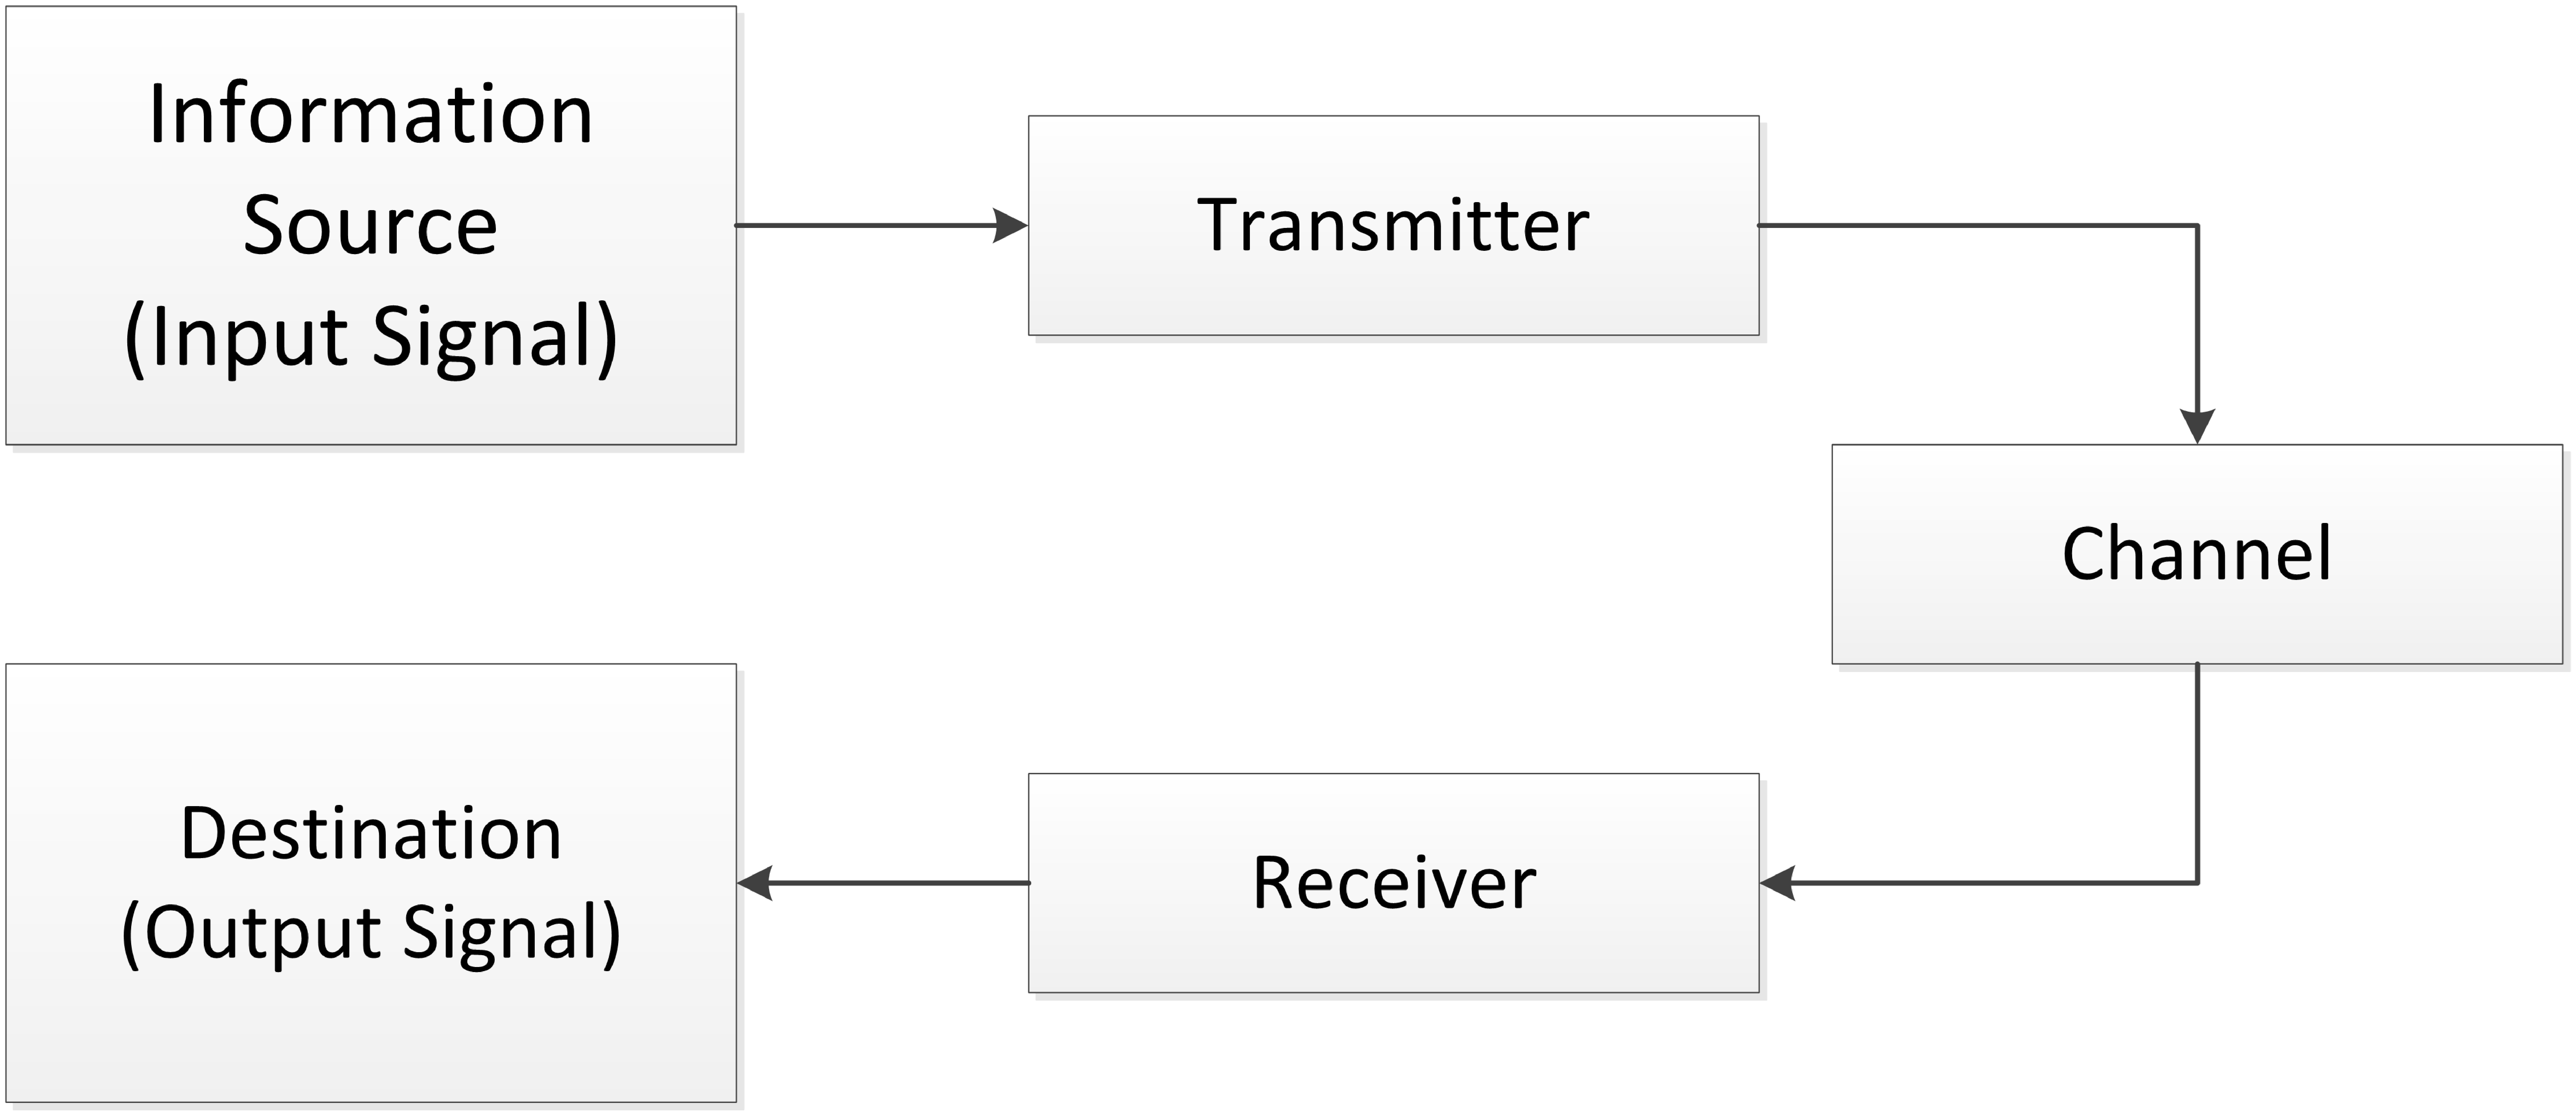
\includegraphics[width=0.65\textwidth]{./figures/digicom_simple}
    \caption{ A simple digital communication system block diagram.
    \label{fig:digicomsimple}}
\end{figure}

The transmitter is located at one point in space, the receiver is located at
some other point separate from the transmitter, and the channel is the medium
that provides the electrical connection between them. The former (transmitter),
in particular, is designed aiming to produce waveforms suitable for transmission
over the channel, a waveform. In the receiver the signal is normally corrupted
version of the transmitted signal, which is due to channel imperfections, noise
and interference. The receiver is designed to reconstruct a recognizable form of
the original message signal and to deliver it to a destination.

\section{Elements of Digital Communications Systems}

%block diagram of a digital communication system
\begin{figure}[htbp]
    \centering
    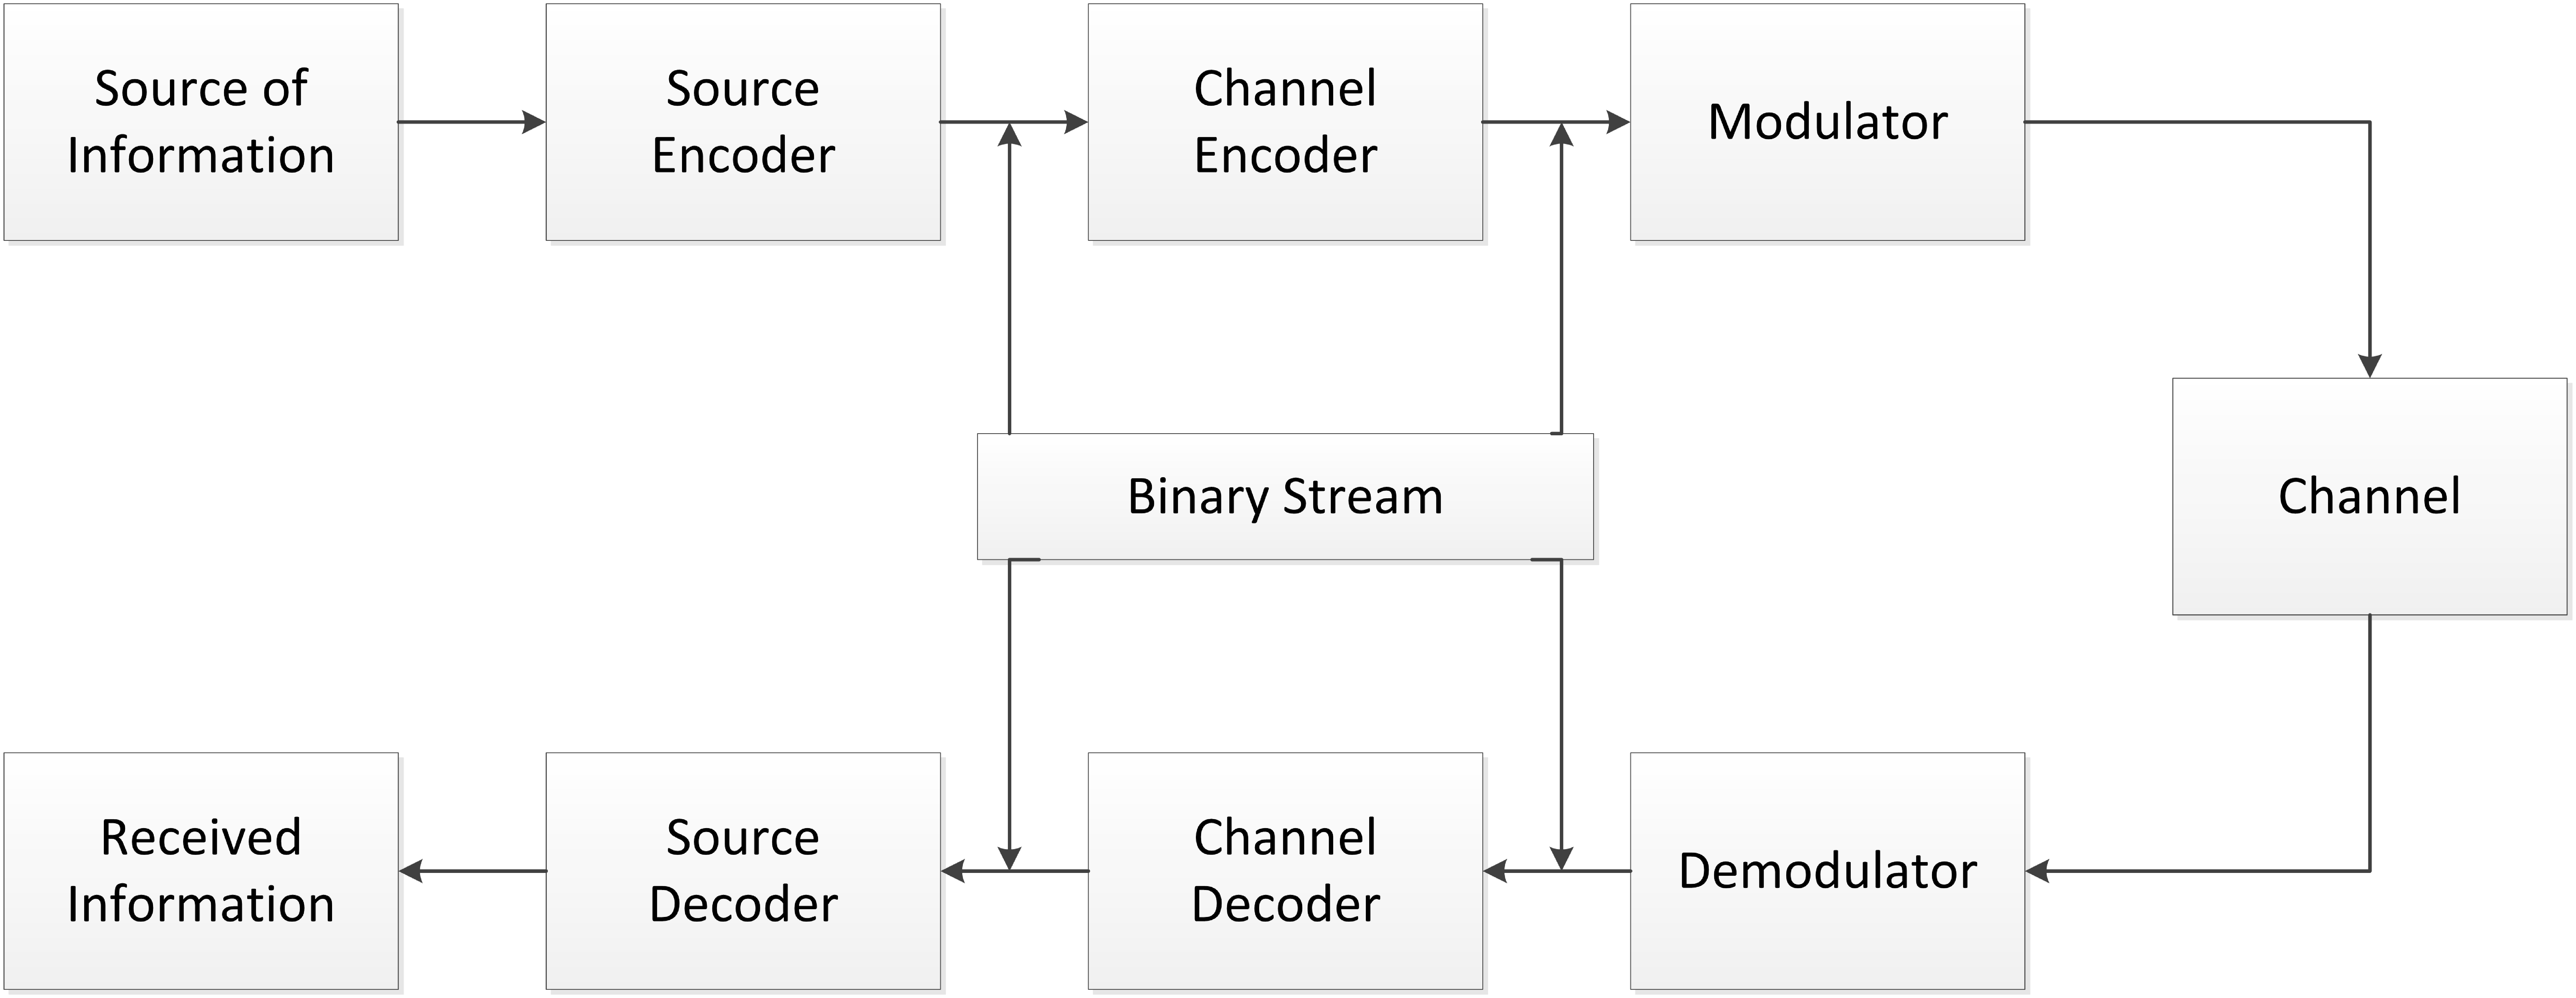
\includegraphics[width=0.85\textwidth]{./figures/digicom_bd}
    \caption{ Digital communication system block diagram.
    \label{fig:digcombd}}
\end{figure}

\subsection{Source of information}

The sources of information can be of two main kinds, \emph{analog information
sources} and \emph{digital information sources}. Analog information sources can
be human like voice, or natural like a humming bird. However, since Digital
communication systems work with a discrete and finite alphabet of symbols such
signals have to be converted to digital information prior to any process. Any
device that can record images or voice from the real world and can reproduce
back is making such analog to digital an digital to analog conversions
respectively.

Digital information sources are basically any information that was not
recorded or generated in the real world, it was generated by a software in a
PC. For example a digital painting or a 3D model.

\subsection{Source Encoder / Decoder}

The \emph{source encoder}  and \emph{source coder} converts the input symbol
sequence into a binary sequence (0 and 1) by assigning codewords to the symbols
in the input sequence. Basically the source encoder input is a analog waveform
and it samples, quantize and compress this analog waveform to a binary message
\cite{ocw:digicomm}.

At the receiver, the \emph{source decoder} converts the binary output of the
channel decoder into a analog waveform, doing the opposite operations of the
\emph{source encoder}. The decoder for a system using fixed length code words is
quite simple, but the decoder for a system using variable length code words can
be very complex \cite{ocw:digicomm}.

Aim of the source coding is to remove the redundancy in the transmitting
information, so that bandwidth required for transmission is minimized. This
approach is based on the probability of the symbol codeword is assigned. The
higher the probability, the shorter the codeword.

\subsection{Channel Encoder / Decoder}

Error control is accomplished by the channel coding operation that consists of
systematical addition of extra bits to the output of the source coder. These
extra bits do not convey any information but helps the receiver to detect and/or
correct some of the errors in the information bearing bits. There are two
methods of channel coding, the \textit{Block Coding} and \textit{Convolution
Coding}.

In the block coding method the encoder takes a block of ‘k’ information bits
from the source encoder and adds ‘r’ error control bits, where ‘r’ can be chosen
based on ‘k’ and error control capabilities desired, this process is
accomplished by a matrix multiplication and that is the origin of the "block" in
block coding. In the convolution coding process the message goes through a
sequence of tapped-delay line operations which works in the same way as
convolving the message with the impulse response of the code, with modulo-2
operations.

The Channel decoder recovers the information bits from the coded binary stream,
error detection and possible correction is also performed by the channel
decoder.

\subsection{Modulator}

The modulator converts the input bit stream into a waveform suitable for
transmission over the communication channel. Advanced modulation schemes such as
Orthogonal Frequency Division Multiplexing (OFDM) can be effectively used to
minimize the effects of channel noise to match the frequency spectrum of
transmitted signal with channel characteristics.

\subsection{Demodulator}

The extraction of the message from the information bearing waveform produced by
the modulation is accomplished by the demodulator. The output of the demodulator
are symbols which can be detected and the converted to bits to form a received
message.

\subsection{Channel}

The Channel is the medium of wave propagation (wireless in this work) then
creating a "connection" between transmitter and receiver. The different channels
are: pair of wires, coaxial cable, optical fiber, radio channel, satellite
channel or combination of any of these.

\section{Additional Modules}

%augmented block diagram
\begin{figure}[htbp]
    \centering
    
\includegraphics[width=0.85\textwidth]{./figures/digicom_plus}
    \caption{ Digital communication system block diagram with additional blocks.
    \label{fig:digicomplus}}
\end{figure}

Some additional blocks as shown in the block diagram  at Figure \ref{fig:digicomplus}
are used in most of digital communication system:

\begin{itemize}

  %\item \textbf{Encryptor:} Encryptor prevents unauthorized users from
    %understanding the messages and from injecting false messages into the system.

  \item \textbf{Multiplexer:} Multiplexer is used for combining signals from
different sources so that they share a portion of the communication system.

  \item \textbf{Demultiplexer:} DeMultiplexer is used for separating the different
signals so that they reach their respective destinations.

  %\item \textbf{Decryptor:} It does the reverse operation of that of the Encryptor.

\end{itemize}

\subsection{Synchronization}

Synchronization involves the estimation of both time and frequency. Coherent
systems need to synchronize their frequency reference with carrier in both
frequency and phase (carrier recovery). The synchronization begins with the
Automatic Gain Control (AGC) which scales the received waveform to a know power
level, then the timing recovery or carrier recovery process can be executed.

Timing or symbol recovery is the process of by with the receiver estimates the
symbol frequency of the received waveform, that process results in the best time
instants to sample a received waveform. Timing recovery is a requirement of all
digital communication systems \cite{akbook}.

Carrier recovery is a processes used in both coherent and non-coherent
demodulation where the phase and the frequency of the transmitter carrier wave
are recovered by the receiver and thus after having such information it is
possible to extract the information in the transmitted signal. Considering that
the phase and frequency of the transmitted wave probably will be affected by
noise, it is not a straight-forward method, it includes filtering and usually
feedback systems (PLLs) to correct the errors in phase or frequency caused by
the noise.
